\section{Approach}
\label{sec:method}

% [R01]
This section presents how PyTT detects Python type errors by tracking
conditional type-state changes across function calls. We first explain
the overall workflow and the function contracts used to represent these
changes. We then describe how PyTT extracts the contracts from code,
uses them to check operations, and investigates the resulting conflicts.

\subsection{Overview}

\begin{figure}[!htbp]
\centering
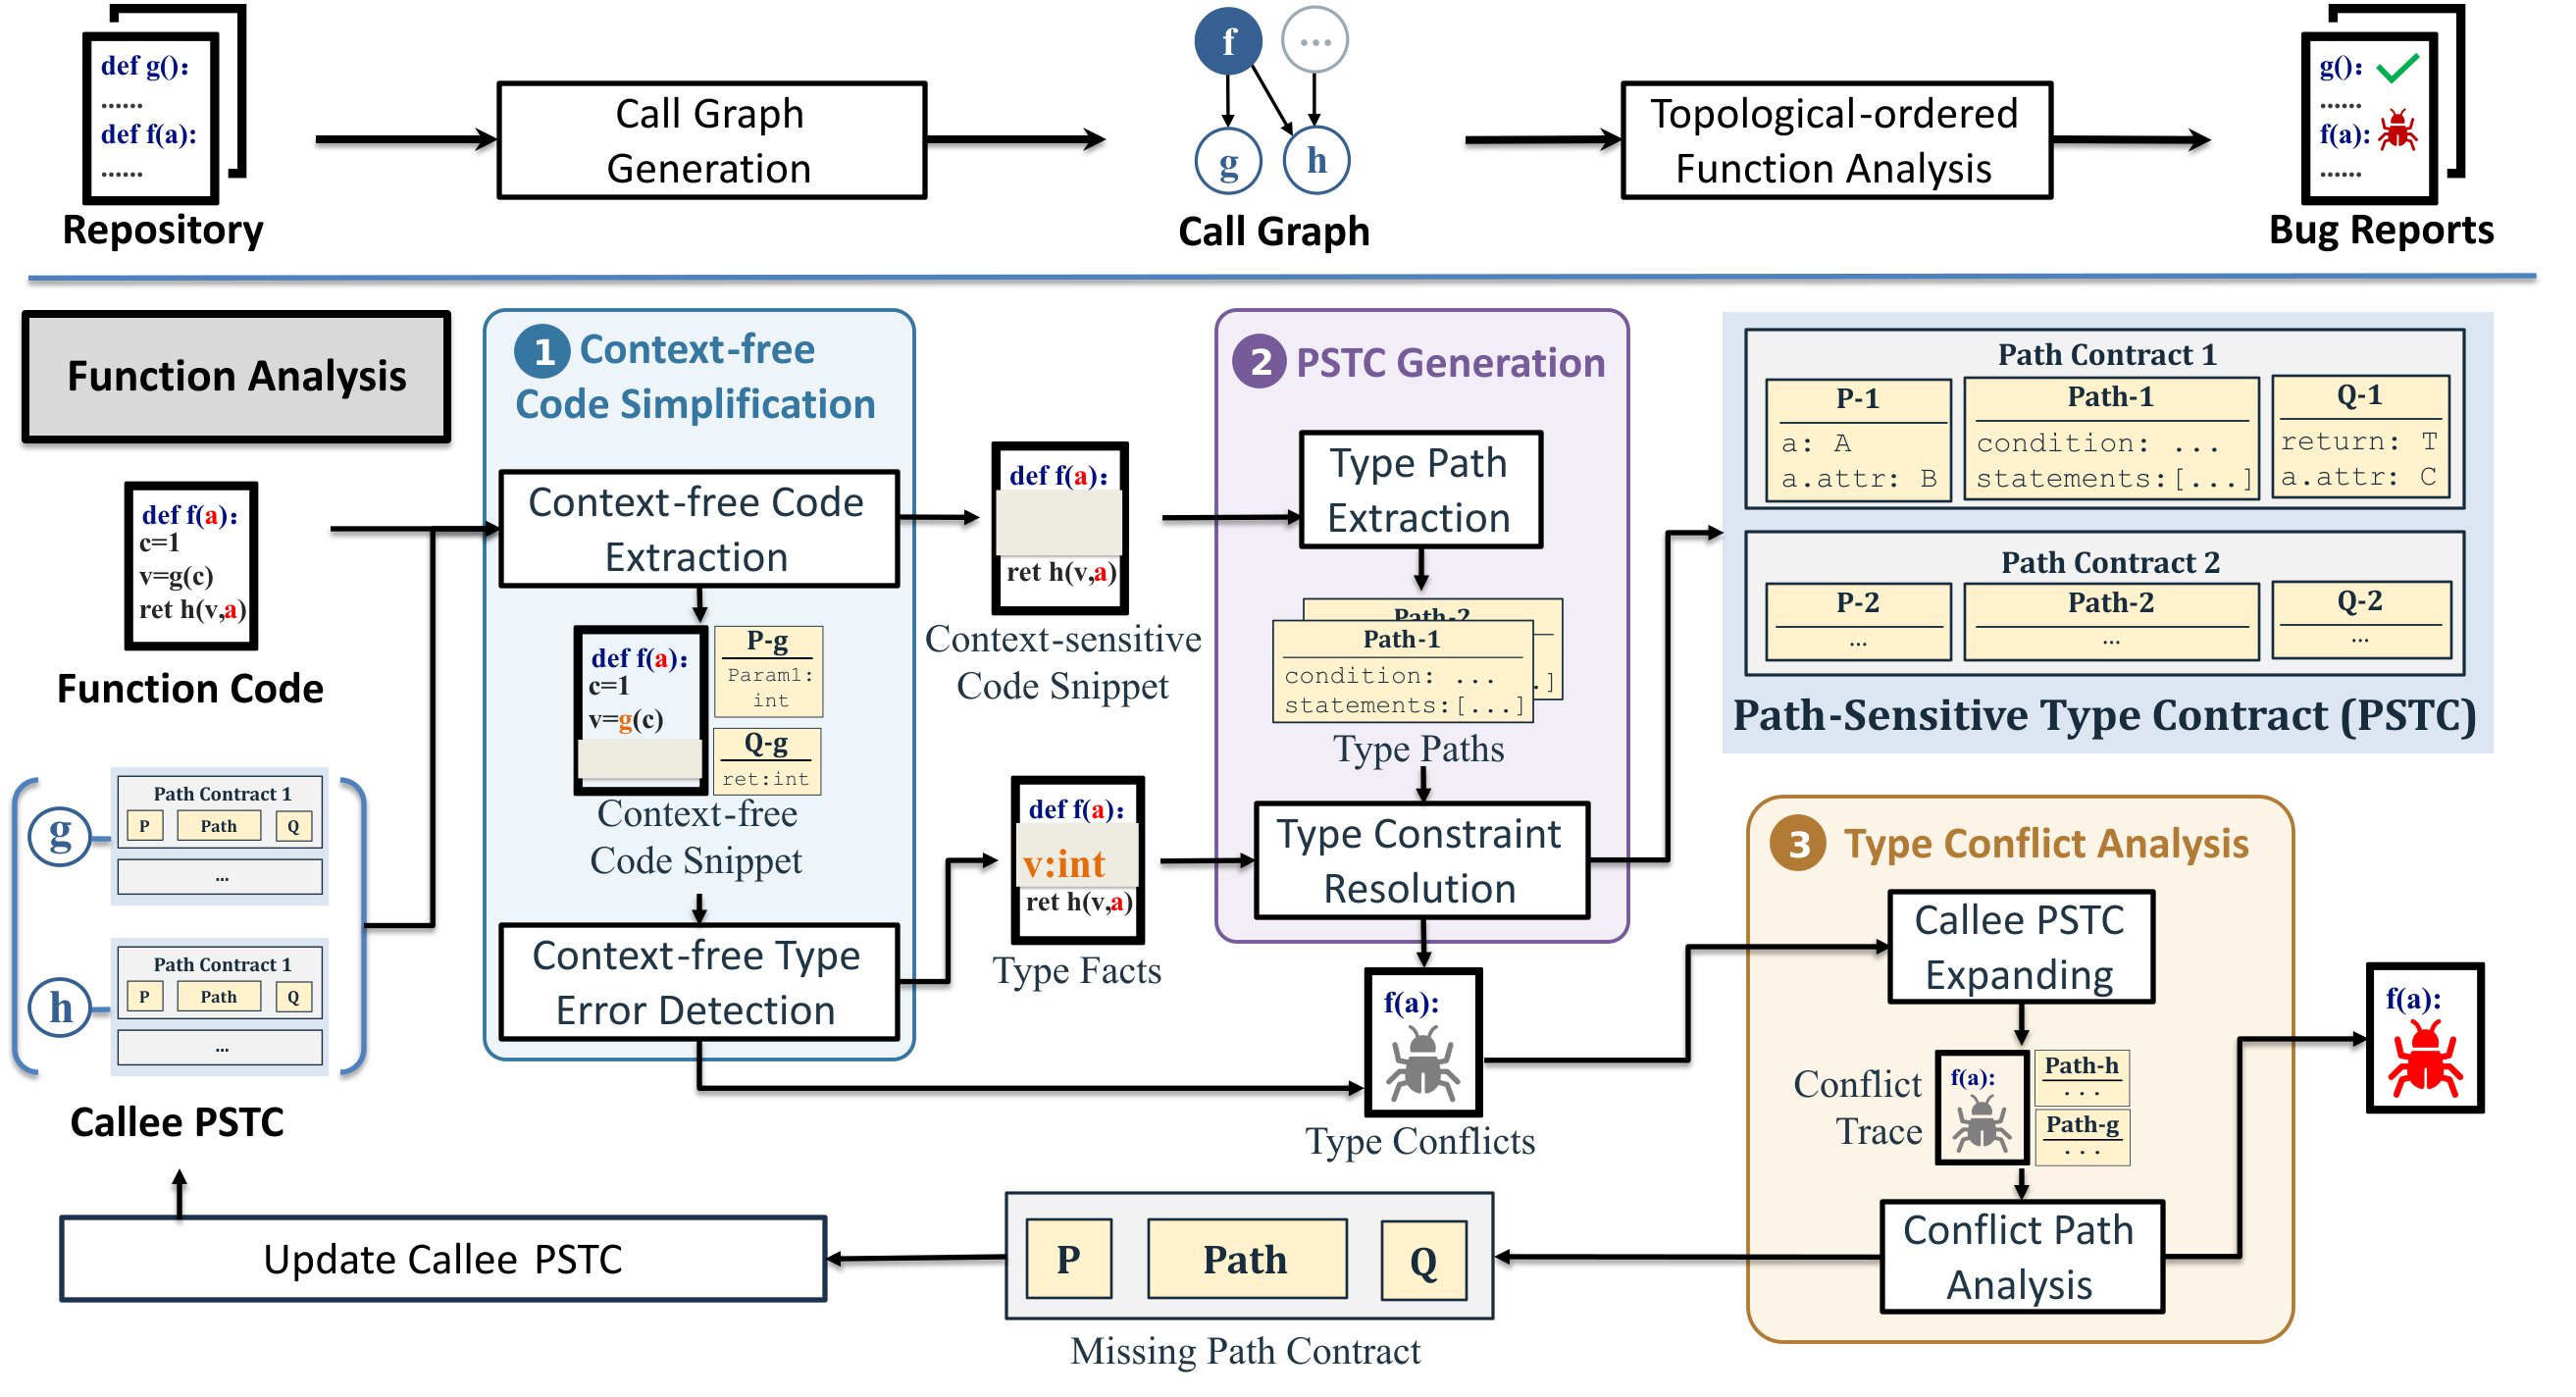
\includegraphics[width=\linewidth]{photos/methodOverview.png}
\caption{Overview of PyTT's workflow}
\label{fig:method-overview}
\end{figure}

% [R02]
To check an operation after a function call, PyTT needs the types
established by that call under the current calling conditions. It records
this information in a \emph{path-sensitive type contract} (PSTC), which
relates a function's entry conditions to its return value and shared-state
updates along different paths. A caller can use the relevant contract
cases to update its type-state and check subsequent operations.

Figure~\ref{fig:method-overview} shows how PyTT constructs and uses these
contracts for a Python repository. PyTT builds a call graph and gives
priority to analyzing callees, whose contracts then provide information
for analyzing callers. For each function, it performs three phases.

% [R03]
\textbf{(1) Context-free Code Simplification.}
Analyzing a function under different calling conditions can repeat work
on computations whose type behavior is already determined. PyTT first
identifies and checks these computations using static analysis. It then
reuses their type facts when analyzing the remaining code, reducing the
work needed to consider different paths.

% [R04]
\textbf{(2) PSTC Generation.}
The remaining code can produce different types under different entry
conditions. PyTT extracts these conditional transitions by identifying
explicit paths with static analysis and inferring implicit paths with an
LLM. It combines the requirements and effects along each path with the
facts from Phase~I and available callee contracts. The resulting PSTC
records the transitions used to check operations in callers.

% [R05]
\textbf{(3) Type Conflict Analysis.}
A conflict found using an inferred contract may reflect either a program
error or an inaccuracy in that contract. To distinguish them, PyTT traces
the conflicting type facts to the relevant caller and callee paths and
analyzes those paths under the calling conditions. It reports errors
supported by this analysis and corrects contracts responsible for false
alarms. Cases with insufficient evidence remain unresolved.

% [R06]
These phases are connected through the contracts they construct and
revise. A callee contract is used to analyze its callers; a correction to
that contract can therefore change their analysis results. PyTT repeats
the affected analyses until no pending work remains or the configured
budget is reached. It then reports confirmed type errors and records
undecided cases as unresolved. The PSTC model addresses Challenge~1 in
the introduction, its extraction in Phases~I and II addresses
Challenge~2, and conflict analysis in Phase~III addresses Challenge~3.

\subsection{Design of Path-Sensitive Type Contracts}
\label{sec:state-model}

% [R07]
The motivating example establishes two requirements for a function
summary. It must describe the change of type to values shared with the caller, and
it must retain the conditions under which each change occurs. 
PyTT therefore needs a summary that connects the incoming type-state and
execution conditions to the types established by the call.

\subsubsection{Representing Calling Conditions and Updates}

% [R08]
To express changes beyond the return value, the summary must refer to the
variables and attributes read or updated by the function. PyTT represents
their type information at a program point as a \emph{type-state}
\[
    S:L\rightarrow\mathcal{T},
\]
where $L$ contains the tracked locations and $\mathcal{T}$ is the domain
of type information, including sets of possible types. A location can be
a parameter, a local or global variable, or a class or instance
attribute. A distinguished result location records the return value on
normal exit. Thus, $S(\ell)$ describes the type information for the value
held at location $\ell$. An assignment to an attribute changes the facts
for that attribute's contents. If the caller and callee refer to the
same object, this update also changes the facts used when the caller
next reads the attribute.

% [R09]
The summary must also specify when these post-call facts apply. PyTT
expresses this information using \emph{state assertions}, which describe
sets of states through type facts, branch conditions, and relevant
object-identity constraints. An entry assertion can require a string
message body and a \texttt{Utf8Encoder} argument, while an exit assertion
can state that the body holds bytes after normal return. Associating
these assertions keeps the resulting field type connected to the
calling condition that establishes it. Branch conditions remain relevant
because identical entry types need not imply identical execution paths.

\subsubsection{Connecting Assertions through Execution Paths}

% [R10]
Entry and exit assertions describe the conditional change needed by a
caller. To check that change and investigate a conflict, PyTT also needs
to retain the operations that produce it. For example, an exit assertion
that the message body holds bytes does not show which call produced the
bytes or which assignment stored them. PyTT therefore associates each
pair of assertions with a path description. This description records
guards, operation requirements, calls, and updates in execution order.
It includes explicit branch choices and implicit choices of behavior
that depend on operand types.

% [R11]
These three components form a path contract $(p,m,q)$, where $p$ is the
entry assertion, $m$ is the path description, and $q$ is the exit
assertion. A function can have several such cases, collected in its PSTC
\[
    \mathit{PSTC}(f)\subseteq
    \mathcal{A}\times\mathcal{M}_f\times\mathcal{A},
\]
where $\mathcal{A}$ is the set of state assertions and
$\mathcal{M}_f$ is the set of path descriptions for $f$. Each case keeps
a particular path associated with its entry conditions and post-call
facts. The PSTC thus represents the information required to transfer
type facts across a call while retaining the behavior behind those facts.

% [R12]
A path contract specializes the Hoare-triple structure introduced in the
background. A correct case states that if execution starts in a state
satisfying $p$, follows $m$, and returns normally, then $q$ holds
afterward. The caller can use these facts under the corresponding
conditions. This partial-correctness interpretation describes normal
returns; it does not guarantee that execution reaches one without a type
error. PyTT checks the operations along the path and tracks their
exceptional continuations separately. Moreover, the cases extracted by
the analysis may contain inaccuracies, which Phase~III investigates when
conflicts arise.

% [R13]
For \texttt{encode\_message}, one case starts with a string body and a
\texttt{TextEncoder} argument. Its path calls the encoder and assigns the
returned string to the body, establishing a string body on normal return.
A second case associates a \texttt{Utf8Encoder} argument with a path that
writes bytes to the body. These two string-input cases both return
\texttt{None} but establish different field types. A third case covers a
non-string input and leaves the body unchanged. Together, the cases show
that the contract must preserve both the incoming condition and the
update established on its path. The next two phases explain how PyTT
obtains this information without repeating the same analysis for every
calling condition.

\subsection{Phase I: Context-free Code Simplification}
\label{sec:extraction}

% [R14]
Constructing the contract defined above requires examining behavior under
different entry conditions and execution paths. When a path contains
calls, its analysis also depends on the relevant paths of the callees,
increasing the number of combinations to consider. Reanalyzing the entire
function for each combination would repeat computations whose type
behavior does not depend on the unknown entry state. PyTT first separates
these computations and analyzes them once, so that subsequent path
analysis can reuse their results.

\subsubsection{Identifying Computations for Shared Analysis}

% [R15]
The first step is to determine which computations can be analyzed in
this way. We call a computation \emph{context-free} when local semantics
and available callee PSTCs determine its type behavior without resolving
the unknown entry type-state. Here, a computation consists of an operation
and the definitions, guards, shared-state accesses, and callee effects on
which its type behavior depends. Starting from the operation, PyTT follows
these dependencies backward. It places the computation in $C_I$ only when
every required type and effect can be resolved from local semantics,
already established facts, or applicable callee PSTCs. If a dependency
reaches an unknown entry value, an unresolved shared-state read, or an
uncovered callee behavior, the affected computation remains in $C_D$, the
\emph{Context-sensitive Code Snippet} in the workflow figure.

For \texttt{f(a)} in Figure~\ref{fig:method-overview}, the assignment
\texttt{c = 1} provides a known integer argument to \texttt{g}. Together
with the depicted PSTC of \texttt{g}, this determines that the result
\texttt{v} is an integer without knowing the type of \texttt{a}. The
computation can therefore be analyzed in $C_I$. The call
\texttt{h(v, a)} still depends on \texttt{a} and remains in $C_D$.
This classification also considers shared-state dependencies of a call;
known argument types alone do not establish that a call is context-free.
For example, a call also remains in $C_D$ when its callee may read or
update a shared location whose incoming contents are unresolved.

\subsubsection{Supplying Type Facts to the Remaining Code}

% [R16]
Separating $C_I$ is useful only if its results remain available where
the rest of the function uses them. PyTT checks $C_I$ using local
operation semantics and callee PSTCs, and supplies the inferred type
facts to their subsequent uses in $C_D$. In the figure, each analysis of
\texttt{h(v, a)} can start with the known integer type of \texttt{v}; it
does not need to infer \texttt{g(c)} again for each possible type of
\texttt{a}. A conflict encountered while checking $C_I$ is passed to
Phase~III, just as a conflict in the remaining code would be.

% [R17]
These facts must remain tied to the execution that establishes them.
A fact produced by an operation applies after that operation succeeds,
and an intervening write can change the contents of the location it
describes. PyTT therefore retains each fact's condition, value or
location version, and supporting source or contract. It also preserves
the source positions and control dependencies of $C_I$ and $C_D$, so
that their checks and updates can later be assembled in execution order.
Branches, shared-state writes, and exceptional continuations in $C_I$
remain part of the summarized behavior. Phase~I thus provides reusable
facts for path analysis without discarding the conditions of their use.
If an intervening operation may overwrite a location and PyTT cannot
identify a disjoint target, it invalidates the reusable fact rather than
carrying that fact into $C_D$.

\subsection{Phase II: PSTC Generation}
\label{sec:pstc-generation}

% [R18]
Phase~I determines the type facts that can be shared across calling
conditions. It does not yet determine the behavior of $C_D$, such as the
result of \texttt{h(v, a)} for different types of \texttt{a}. To construct
a PSTC, PyTT must now associate the remaining behavior with the conditions
under which it occurs. It does this in two steps. Static analysis first
identifies the explicit paths through the source code. The LLM then
infers the type-dependent behavior within those paths, allowing PyTT to
construct their entry and exit assertions.

\subsubsection{Separating Explicit Execution Paths}

% [R19]
Different branches can perform different updates, so combining their
results before recording their conditions would lose information needed
by the contract. PyTT uses static analysis to extract explicit paths
through $C_D$ within the configured bounds. Branch outcomes, exceptional
successors, and bounded loop or recursive unfoldings create explicit path
alternatives. Each path retains its guards and operations in source order,
along with the facts from Phase~I available at each use. These are the
initial \emph{Type Paths} in Figure~\ref{fig:method-overview}. When a bound
stops exploration, PyTT records the remaining frontier as uncovered; it
does not treat the truncated path as a complete contract case.

In \texttt{encode\_message}, the body test separates the path that calls
the encoder and assigns its result from the path that leaves the body
unchanged. This separation identifies where an update occurs and the
body condition under which it occurs. It does not yet determine the
type of the value returned by the encoder on the updating path.

\subsubsection{Resolving Implicit Paths}

% [R20]
The remaining uncertainty arises because a source operation can select
different behavior for different operand types. The encoder call uses
the implementation provided by its argument; similarly,
\texttt{x + y} can perform arithmetic, concatenate strings, or invoke a
user-defined method. Enumerating source branches alone does not separate
these implicit paths. Their requirements and effects must be determined
to obtain the type-state changes along an explicit path.

PyTT uses an LLM to propose these paths one explicit path at a time. The
input identifies the source operations whose behavior remains unresolved
and supplies the facts established in Phase~I, relevant repository type
information, and applicable callee PSTCs. The requested output separates
the operand-type conditions for each possible behavior from that
behavior's operation requirements, result types, and shared-state effects.
The LLM output is therefore a set of candidate implicit paths, not an
independent error decision. PyTT attaches each proposal to the source
operations and known facts from which it was inferred so that later
composition and conflict analysis can inspect its support.

% [R21]
PyTT combines these results with the ordered checks and updates from
$C_I$ and $C_D$ to form cases $(p,m,q)$. For the updating path of
\texttt{encode\_message}, the return type of each encoder determines the
type stored by the subsequent assignment. Keeping the encoder condition
with that assignment yields a string-body case for \texttt{TextEncoder}
and a bytes-body case for \texttt{Utf8Encoder}. Together with the
unchanged-body path, these cases form the helper's PSTC. Each case
retains its source locations, inference context, and supporting
dependencies, so that the analysis can revisit how its facts were
obtained if they later cause a conflict. If the available proposals do
not cover an operand-type alternative represented by the current entry
state, PyTT requests supplementary analysis when budget remains and
otherwise retains that alternative as uncovered. A missing proposal alone
does not justify either a safe result or an error report.

\subsubsection{Applying Contracts to Check Caller Operations}
\label{sec:composition}

% [R22]
The constructed PSTC describes the callee in terms of its parameters and
the shared locations it accesses. To use it for a particular call, PyTT
must first relate those references to the caller's values and objects.
After evaluating the call target and arguments in source order and
checking argument binding, PyTT constructs a substitution $\theta$ for
this correspondence. For example, the helper's message parameter is
mapped to the message object passed by \texttt{make\_line}.
This instantiation allows an update expressed through the callee's
parameter to affect the same field that the caller later reads.

If two arguments refer to the same object, the substitution preserves
their shared identity. Internal symbols and newly allocated objects are
fresh for each call. These rules keep shared locations connected without
merging objects that belong to different invocations. The same
composition procedure is used when constructing caller contracts and
when analyzing calls under given entry conditions.

% [R23]
After mapping the references, PyTT determines which cases are relevant
to the call. Let $A$ be the caller's abstract state and
$\operatorname{Facts}(A)$ its type facts and path conditions. For a case
$(p_i,m_i,q_i)$, PyTT considers
\begin{equation}
    \operatorname{Facts}(A)\land\theta(p_i).
    \label{eq:applicability}
\end{equation}
The conjunction restricts the calling states to those satisfying the
case's entry assertion. An inconsistent case is excluded. A case that
remains is analyzed under the combined condition, which is retained
with its results. Several cases may apply to different parts of the
calling state; consistency does not show that one case covers every
possible execution. If the available cases leave states uncovered, PyTT
requests further analysis or records those states as unresolved. Lack
of a matching case alone does not establish a type error.

% [R24]
For each relevant case, PyTT follows the instantiated path in execution
order to determine the state used by subsequent operations. Guards
restrict the current condition, reads use the facts for the current
location contents, and writes update those facts. On normal return,
the exit assertion describes the resulting return value and shared
state; it records the effects already processed along the path without
applying them a second time.

A shared-state update must reflect which object is written. If the
write definitely targets one location of a single object, PyTT replaces
its previous type fact with the new one, a \emph{strong update}. If
several targets are possible, a \emph{weak update} retains the possible
old and new contents. Facts about locations known to be unaffected
remain available. An unknown write invalidates precise facts for the
region it may affect. Under this memory abstraction, later checks use
only facts that have survived the call's possible write footprint;
imprecise targets reduce precision instead of silently preserving an
earlier fact.

% [R25]
As PyTT processes each operation, it checks the values used by that
operation against the state established by the preceding steps. For an
operation with requirement $R$ and current facts $F$, it examines the
success condition $F\land R$
and failure condition $F\land\neg R$. These describe the states in which
the operands satisfy or violate the operation's requirement. If the
failure condition is consistent with a represented calling condition,
PyTT creates a candidate conflict and retains the source location and the
facts supporting that condition. If missing types or uncovered behavior
prevent PyTT from establishing either alternative, the check remains
unresolved. Normal continuation uses the success facts, while exceptional
continuation carries the state established up to the failed operation.

% [R26]
At the motivating call, the caller's guard establishes a string body
and the encoder argument is a \texttt{Utf8Encoder} instance. These facts
select the case that writes bytes to the shared body. The following
concatenation is consequently checked with a bytes operand and produces
a bytes/string conflict. Replacing the encoder with
\texttt{TextEncoder} selects the string-body case and satisfies the same
operation requirement. The contract now provides the conditional update
needed to distinguish the calls. Since that contract was inferred,
however, a conflict obtained from it still requires the investigation
described next.

\subsection{Phase III: Type Conflict Analysis}
\label{sec:conflict-analysis}

% [R27]
The preceding phases check operations using type facts propagated from
inferred contracts. If a contract loses a condition or assigns the wrong
type to an update, a caller can receive an inaccurate fact and appear
to perform an invalid operation. Inspecting only the operation cannot
determine whether the program produces the conflicting value or the
contract merely predicts it. PyTT therefore returns to the source
behavior that established the disputed fact and analyzes it under the
calling conditions. This phase first constructs a conflict trace and
then uses that trace to decide whether to report an error or revise a
contract.

\subsubsection{Constructing a Conflict Trace}

% [R28]
Reexamining every callee body would repeat analysis unrelated to the
conflict. The path descriptions and supporting dependencies retained in
the PSTCs allow PyTT to select the relevant behavior. Starting from the
conflicting operation or annotation check, PyTT follows the conditions,
values, and shared-object references that support its type facts. It
uses the contributing callee cases to identify which paths need to be
expanded in the call graph.

PyTT connects those callee paths to the caller fragments leading to the
conflict. The resulting \emph{conflict trace} retains guards, operation
requirements, writes, and exceptional control flow, together with the
call-site bindings established during composition. A write through a
callee parameter can thus be followed to a later read through the
caller's reference. The trace provides the source operations and calling
conditions needed to reassess the disputed transition.

\subsubsection{Distinguishing Errors from Contract Inaccuracies}

% [R29]
Using the expanded trace, PyTT re-infers the type-state changes and
checks the operation or annotation that produced the conflict. This step
differs from initial contract construction in two ways. First, the
candidate conflict fixes the calling conditions, object bindings, and
disputed facts that the analysis must explain. Second, trace expansion
replaces the contributing summarized segments with their relevant source
paths instead of reconsidering every behavior of every callee. The
re-inference therefore asks whether those source operations support the
propagated fact and the failing requirement under the recorded calling
condition.

For the motivating example, the trace connects the string guard to the encoder
call, the field assignment, and the final concatenation. With
\texttt{Utf8Encoder}, the encoder returns bytes and the helper stores
them in the body. The concatenation then raises \texttt{TypeError}, which
escapes \texttt{make\_line}. The trace supports a runtime type-error
report because it explains both how the bytes value arises and why the
operation fails under that calling condition.

Suppose instead that an inaccurate contract predicts a bytes update for
a \texttt{TextEncoder} call. Expanding the encoder's behavior reveals
that it returns the string unchanged. The conflicting bytes fact is
then unsupported by the source behavior. PyTT corrects the contract
under the text-encoder condition and dismisses the resulting false
alarm. If the expanded analysis cannot establish an error or justify a
correction, the candidate remains unresolved.

The re-inference result is not treated as a report merely because it
repeats the initial prediction. A runtime report requires a continuous
trace from a feasible entry condition through the value-producing updates
to an escaping type-related failure. A contract correction instead
requires the expanded source behavior to contradict or refine a specific
condition, type, or object binding in the supporting case. When multiple
expanded alternatives remain possible and support different outcomes,
PyTT preserves them and leaves the candidate unresolved unless subsequent
analysis separates their conditions.

% [R30]
The correction must be recorded in the contract so that subsequent
callers receive the revised transition. PyTT adds or revises the
relevant case, corresponding to the \emph{Missing Path Contract} in
Figure~\ref{fig:method-overview}. Depending on the inaccuracy, this can
restore a condition associated with an update, correct a type
combination, distinguish object-identity cases, or supplement an
uncovered entry case. A correction retains the calling conditions
under which it was established and does not replace cases for other
conditions. Other functions may already have used
the previous case, so updating this contract also requires revisiting
their dependent results, as described in Section~\ref{sec:reuse}.

\subsubsection{Determining What to Report}

% [R31]
The trace must support the kind of error being reported. For a
\emph{runtime type error}, it must reach an operation with incompatible
operand types or unmet protocol requirements and show that the resulting
type-related exception escapes the analyzed entry. For a repository
entry, the trace includes the initialization and calls establishing that
state. For an open entry, the report records the symbolic arguments and
state assumptions under which the failure occurs. If a handler consumes
the exception, PyTT records a handled failure. A corrected contract that
removes the conflict leads to dismissal, while insufficient evidence
leaves the candidate unresolved. Reports retain the trace, re-inference
context and result, and exception disposition.

% [R32]
An \emph{annotation-contract error} concerns whether a declaration agrees
with the behavior of the code. PyTT checks whether declared input types
meet the requirements of the operations using them, and whether returned
or stored values satisfy their declared types. A conflict undergoes the
same tracing and contextual re-inference as an operation conflict. A
confirmed report identifies the declaration, the incompatible case, and
the supporting behavior. Because the claim concerns the declaration's
agreement with the code, it does not require a repository call that
raises an exception. This separates the evidence needed for annotation
conflicts from the runtime failures described above.

\subsection{Interprocedural Refinement and Reuse}
\label{sec:reuse}

% [R33]
Phase~III can correct a callee contract, but that correction alone does
not update results already computed for its callers. PyTT records the
contract dependencies of those results so that it can identify which
analyses need to be repeated. When a PSTC changes, PyTT assigns it a new
version, invalidates results that used its previous version, and
re-enqueues the affected caller entries. Reanalysis can in turn change
their contracts and propagate the correction to further callers.
Algorithm~\ref{alg:analysis} summarizes this feedback through a worklist
of functions and their calling states.

\begin{algorithm}[t]
\caption{PSTC propagation and conflict-driven refinement}
\label{alg:analysis}
\begin{algorithmic}[1]
\Require Repository $P$, fixed call graph $G$, entries $E$, budgets $B$
\Ensure Runtime reports, annotation-contract reports, and unresolved cases
\State Initialize PSTCs and a callee-first worklist $W$ from $G,E$
\While{$W\neq\emptyset$ and analysis budget remains}
  \State Remove a function entry $(f,A)$ from $W$
  \State Partition entry-independent computations and infer reusable facts
  \State Extract bounded explicit paths and propose their implicit alternatives
  \State Construct or supplement $\mathit{PSTC}(f)$; retain uncovered states
  \State Compose PSTCs under $A$ and collect candidate conflicts
  \For{each candidate conflict $c$}
    \State Trace supporting conditions, values, object identities, and callee cases
    \State Expand relevant paths and re-infer behavior in the calling context
    \If{the trace supports an escaping runtime failure}
      \State Record a runtime report for $c$
    \ElsIf{the trace supports an annotation--behavior incompatibility}
      \State Record an annotation-contract report for $c$
    \ElsIf{the trace supports a correction to a PSTC case}
      \State Revise the PSTC and invalidate dependent results
      \State Enqueue affected caller entries in $W$
    \Else
      \State Retain $c$ as unresolved
    \EndIf
  \EndFor
\EndWhile
\State Retain uncovered states and undecided candidates as unresolved
\end{algorithmic}
\end{algorithm}

% [R34]
Repeated analysis also creates opportunities to reuse work that remains
applicable. The facts from Phase~I, common path prefixes, and callee
PSTCs can serve multiple cases and callers. Reusing a PSTC still requires
instantiating its references and refreshing internal symbols for the
current call. Reusing an already computed call result additionally
requires matching its relevant entry state, object identities, call
targets, analysis assumptions and settings, exploration bounds, and
supporting contract versions. These conditions tie reuse to the facts
on which the result depends. The check includes dependencies of reads,
checks, and updates; instances with unknown read or write locations are
recomputed. A cached failure is reconsidered under the current entry's
reachability and exception handling.

% [R35]
Reuse reduces repeated work but does not remove the growth in path
combinations. PyTT bounds path exploration, loop and recursive expansion,
and conflict refinement. Refinement of a candidate stops when its
outcome is established, no new evidence is obtained, or its budget is
exhausted. Unexamined continuations, uncovered states, and undecided
conflicts remain unresolved. The complete cost includes shared fact
inference, path construction, call-site composition, trace expansion,
contextual re-inference, and dependency maintenance, including caller
reanalysis after corrections. Section~\ref{sec:rq2} evaluates this cost
and examines reuse in comparison with direct function-body analysis.
